\section{$H_{\infty}$ Control Design}
In this section we show how to design a $H_{\infty}$ controller for this system. The augmented plant consists in three shaping functions which are in charge of designing the closed loop sensitivity, complementary sensitivity and effort sensitivity; look at Appendix for further details on $H_\infty$.\\

\begin{figure}[h]
	\setlength{\belowcaptionskip}{-10pt}
	\centering
	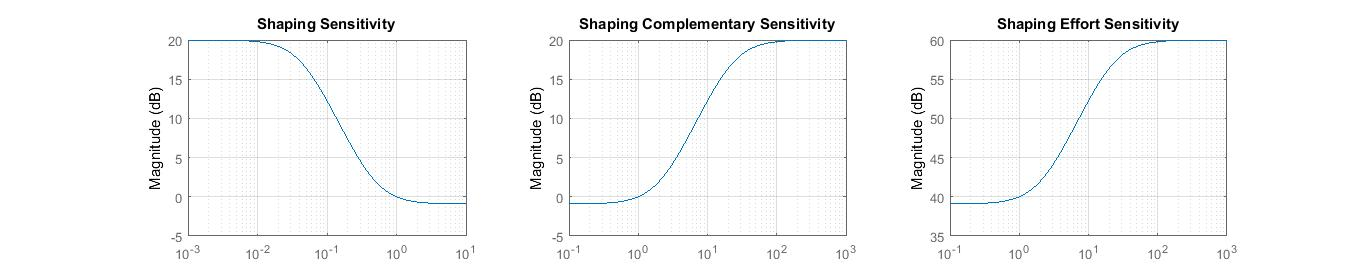
\includegraphics[scale=0.5]{img/hinf_shapes.jpg}
	\caption{Shaping functions.}
\end{figure}

Each function has three degrees of freedom: low frequency gain, cross-over frequency and high frequency gain. The most important one is the cross-over frequency which defines the closed loop bandwidth of the system; in our case, we are aiming at a response time of about one second which corresponds to a cross-over frequency of 1 Hz ($\omega =2\pi $ \SI{}{\radian \per \second}). The gains are tuned so to obtained the desired static error at regime, since we are not including any integral action; the higher the gain the smaller the static error will be. The crucial function in our application is the sensitivity wrt the control input because our actuator constrains us to work in the range $\pm 5V$; hence, we need to give more weight to penalize the control effort and obtain a feasible action; this last process is performed by an iteration process of trial and error: given a shape, we test the correspondant controller on simulink and check how the control input behaves; if the input saturate then we need to weight more the effort.\\

The controller output of the $H_{\infty}$ design has as many poles as the augmented plant; in our case, the plant has 3 poles (two from the cart and one from the motor) and so the shaping functions (one pole each), thus the final controller is a 6th order transfer function. Since we previously saw that the loopshaping technique achieves good performances with a 3rd order, it is interesting to investigate the option of reducing the complexity of the controller. With this aim, we compute the singular values of the Hankel matrix in order to see how much information is contained by every degree. It turns out that only the first order of complexity brings enough information and can approximate the controller in the bandwidth of interest. In practice, approximating to the third order is a robust solution which will not perturb for sure the theoretical results.\\

  \begin{figure}[h]
  \centering
  \subfloat[Singular values of the Hankel matrix.]
  {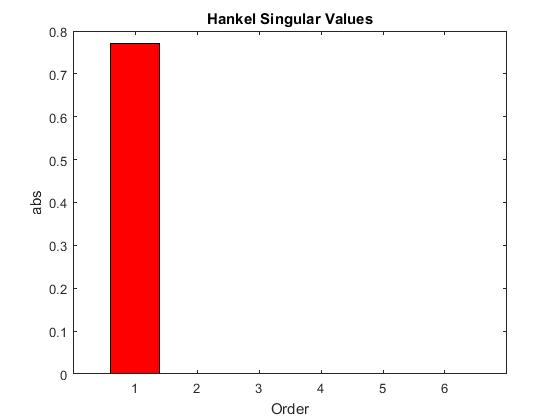
\includegraphics[width=0.49\textwidth]{img/hinf_hankel.jpg}}
  \hfill
  \subfloat[Approximation with only the first order.] {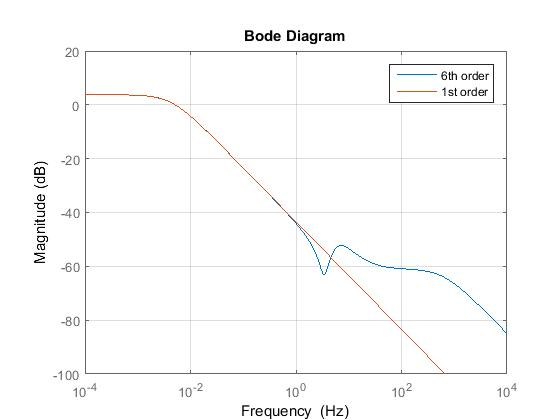
\includegraphics[width=0.49\textwidth]{img/hinf_reduced.jpg}}
  \caption{}
\end{figure}

The downside of this controller is that it does not have any integral action, but this can be easily fixed by moving the slowest pole (of the controller) to zero. This way we are introducing an integral action without affecting the other properties of the designed controller. In Matlab this can be done by converting the state-space model of the controller into a \emph{zpk} model and by literally editing the slowest pole into zero.\\

%\begin{figure}[h]
%\centering
%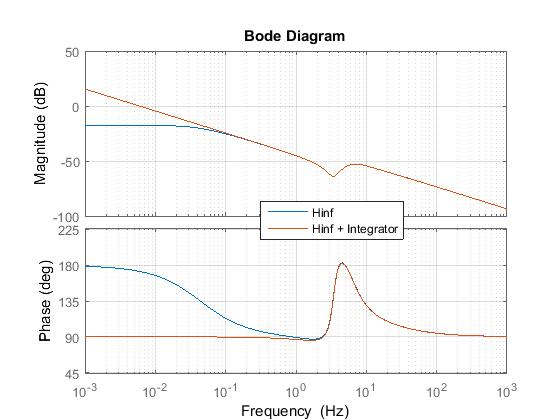
\includegraphics[width=0.5\textwidth]{img/hinf_integrator.jpg}
%\caption{Introduction of the integral action into the controller.}
%\end{figure}

  \begin{figure}[h]
  	\centering
  	\subfloat[Introduction of the integral action into the controller.]
  	{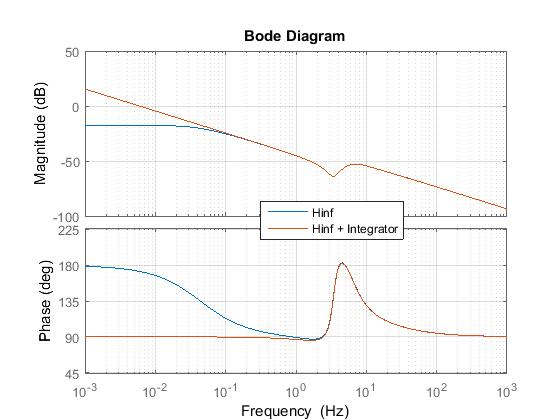
\includegraphics[width=0.49\textwidth]{img/hinf_integrator.jpg}}
  	\hfill
  	\subfloat[Singular values of the Hankel matrix for the controller with integral action.] {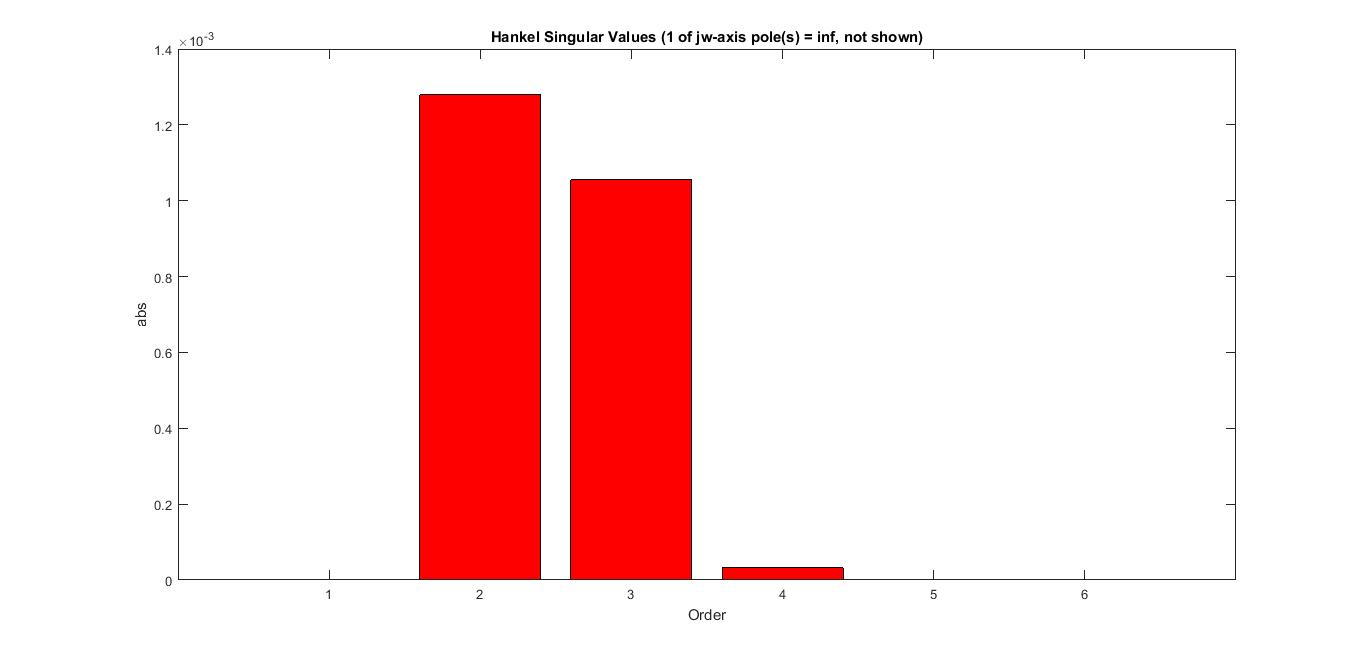
\includegraphics[width=0.49\textwidth, height=180pt]{img/hinf_hankel_int.jpg}}
  	\caption{}
  \end{figure}

Again, we can apply a system reduction to the controller by analizing the singular values of the Hankel matrix. This time the minimum order to get a good approximation is 3, and the bode diagram perfectly overlaps the original one.\\

%\begin{figure}[h]
%\centering
%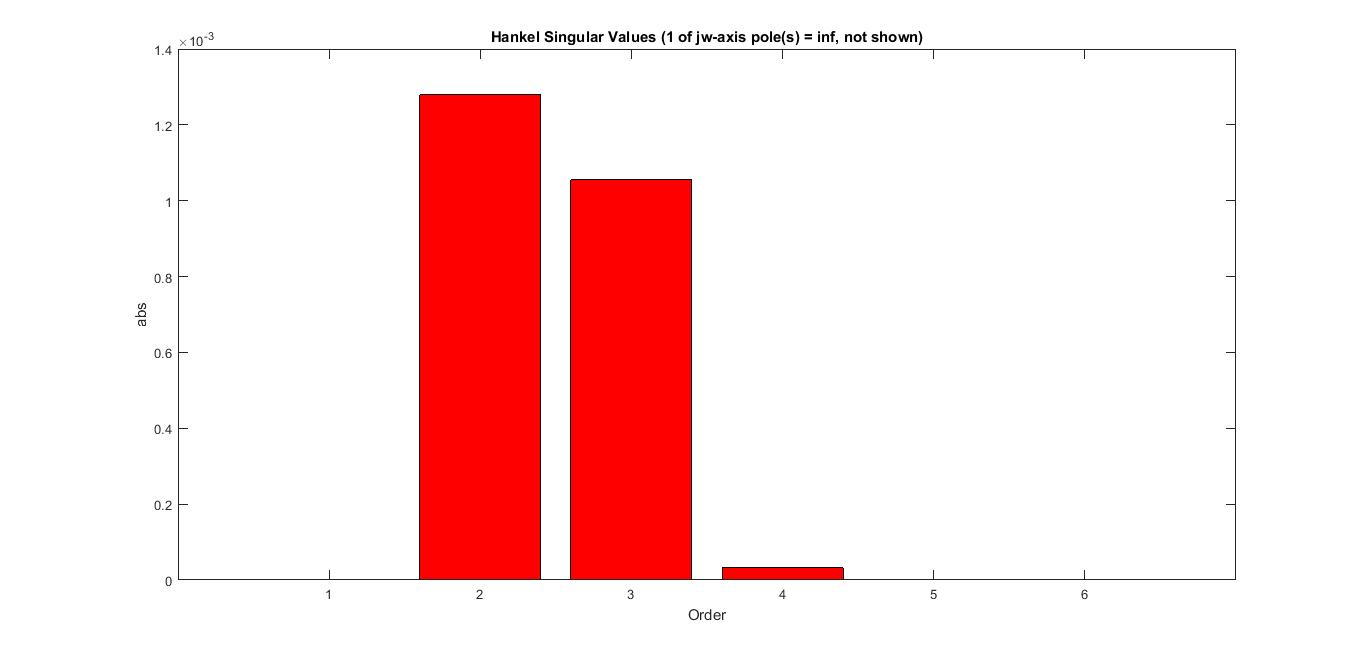
\includegraphics[width=0.5\textwidth]{img/hinf_hankel_int.jpg}
%\caption{Singular values of the Hankel matrix for the controller with integral action.}
%\end{figure}

\begin{figure}[h]
	\centering
	\subfloat[$H_{\infty}$ without integrator]
	{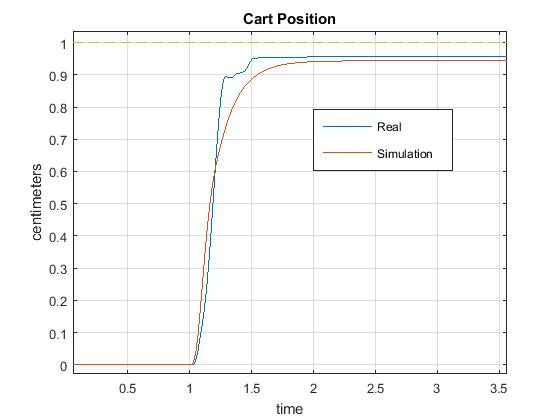
\includegraphics[width=0.49\textwidth]{img/hinf_response_noint.jpg}}
	\hfill
	\subfloat[$H_{\infty}$ with integrator.]{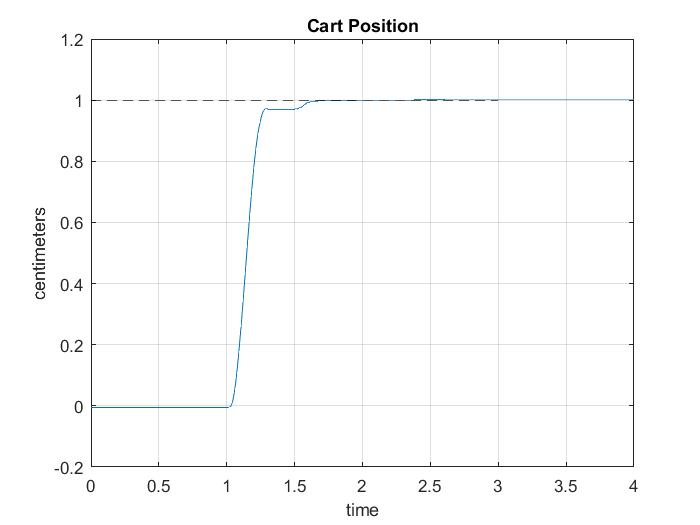
\includegraphics[width=0.49\textwidth]{img/hinf_response_int.jpg}}
	\caption{Comparison between step response of $H_\infty$ controller.}
\end{figure}

  \begin{figure}[h]
  \centering
  \subfloat[$H_{\infty}$ without integrator]
  {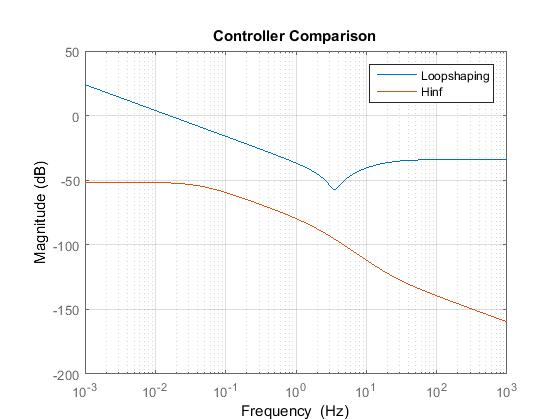
\includegraphics[width=0.49\textwidth]{img/hinf_ls.jpg}}
  \hfill
  \subfloat[$H_{\infty}$ with integrator.]{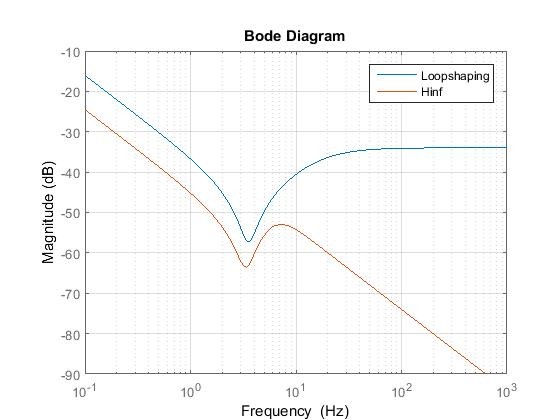
\includegraphics[width=0.49\textwidth]{img/hinf_integrator_ls.jpg}}
\caption{Comparison between Loopshaping and $H_{\infty}$.}
\end{figure}

We now focus on the step responses of the designed controller. It is interesting to see the difference between the design with and without integral action. As it is expected the integrator guarantees zero steady state error and gives better overall performance. The final controller obtained is not much different from the one designed by loopshaping as it is easy to see by plotting the bode diagrams; in particular the $H_\infty$ solution gives more attenuation for higher frequencies.\\

